% =====================================================================
\section{Local theory: the Maclaurin expansion and the radius of
convergence}\label{sec:maclaurin}
% =====================================================================

The sandwich theorem controls the global position of $\Tah$; we now zoom
in on the origin, where the three normalizations
$\Tah(0) = \Tah'(0) = 1$, $\Tah''(0) = 0$ of
Proposition~\ref{prop:derivatives} suggest a degenerate local structure.
The degeneracy is real, and it is the entrance to a chain of
consequences: an inflection with third-order contact, a clean
convexity dichotomy, and a Maclaurin series whose radius of convergence
is set by a pair of complex critical values of $f$, reached through a
picture (Figure~\ref{fig:slit}) that we find to be one of the prettiest
by-products of the theory.

\subsection{The series}

\begin{theorem}[Maclaurin expansion; the quadratic term vanishes]
\label{thm:maclaurin}
The Tahawus function is real-analytic at the origin, and
\begin{equation}\label{eq:maclaurin}
\begin{split}
    \Tah(y) \;=\; 1 + y - \frac{y^{3}}{2} + \frac{y^{4}}{6} +
    \frac{y^{5}}{2} - \frac{49\,y^{6}}{120} - \frac{5\,y^{7}}{9} \\[2mm]
    \qquad + \frac{4313\,y^{8}}{5040} + \frac{49\,y^{9}}{90} -
    \frac{6341\,y^{10}}{3780} - \frac{11549\,y^{11}}{50400} +
    \frac{62041117\,y^{12}}{19958400} + O(y^{13}) .
\end{split}
\end{equation}
In particular the coefficient of $y^{2}$ vanishes identically: $\Tah$
has third-order contact with its tangent line $1+y$ at the origin.
All coefficients are rational numbers.
\end{theorem}

\begin{proof}
Write $u := x - 1$ and recall from \eqref{eq:f-series} that
\begin{equation}\label{eq:phi-def}
    y \;=\; f(1+u) \;=\; u\,\varphi(u),
    \qquad
    \varphi(u) \;:=\; \frac{f(1+u)}{u}
    \;=\; 1 + \frac{u^{2}}{2} - \frac{u^{3}}{6} + \frac{u^{4}}{4} -
    \frac{7u^{5}}{40} + \cdots,
\end{equation}
a power series with $\varphi(0) = f'(1) = 1 \ne 0$. The
Lagrange--B\"urmann inversion formula applied to $y = u\,\varphi(u)$
gives
\begin{equation}\label{eq:lagrange}
    u(y) \;=\; \sum_{n \ge 1} \frac{y^{n}}{n}\,
    [u^{\,n-1}]\,\varphi(u)^{-n},
    \qquad\text{so that}\qquad
    \Tah(y) \;=\; 1 + \sum_{n \ge 1} d_{n} y^{n},
    \quad d_{n} := \frac{1}{n}[u^{\,n-1}]\,\varphi(u)^{-n},
\end{equation}
with positive radius of convergence, since $\varphi(0) \ne 0$. Each
$d_n$ is a rational number, because the coefficients of $\varphi$ are
rational: they are obtained from the exact expansion
$E(u) := (1+u)\ln(1+u) = \sum_{k\ge1} (-1)^{k+1}u^{k}/(k(k-1))$ by
exponentiating ($x^{x} = \exp E$), dividing by $1+u$, and reverting;
all steps are rational recurrences, reproduced in
Appendix~\ref{sec:computational}, which is how the twelve coefficients
displayed in \eqref{eq:maclaurin} were computed exactly. The vanishing
of $d_2$ was already proved in Proposition~\ref{prop:derivatives} via
$\Tah''(0) = -f''(1)/f'(1)^{3} = 0$; it can also be read off directly
from \eqref{eq:phi-def}, since $\varphi$ itself has no linear term, so
$\varphi^{-2}$ has no $u^{1}$-term. As a numerical check, the partial
sum of \eqref{eq:maclaurin} through $y^{12}$ was evaluated against the
directly computed value of $\Tah$: the differences are
$3.2 \times 10^{-11}$ at $y = 0.15$, $3.3 \times 10^{-7}$ at
$y = 0.3$ and $7.0 \times 10^{-5}$ at $y = 0.45$, consistent with a
twelve-term truncation of a series of radius $R \approx 0.65$
(Subsection~\ref{subsec:radius} below).
\end{proof}

\begin{remark}[why the quadratic term vanishes]\label{rem:why-vanishing}
The cancellation has a transparent cause in the two-term decomposition
\eqref{eq:f-two-terms}, $f(x) = x^{x-1} - 1/x$. At $x = 1+u$,
\[
    x^{x-1} \;=\; (1+u)^{u} \;=\; \exp\!\bigl(u\ln(1+u)\bigr)
    \;=\; 1 + 0\cdot u + u^{2} - \frac{u^{3}}{2} + \cdots,
    \qquad
    \frac{1}{x} \;=\; 1 - u + u^{2} - \cdots,
\]
and the two terms have \emph{identical quadratic parts} $+u^{2}$, which
cancel in the difference, while their linear parts differ by exactly
$u$. So $f$ is ``linear plus cubic'' at $x=1$, and reversion preserves
the pattern: $\Tah$ is ``linear plus cubic'' at $y = 0$. Neither
$\ee^{y}$ nor $1 + y + cy^{2}$ with $c \ne 0$ shares this property; in
the two-parameter family of functions with $\Tah(0)=\Tah'(0)=1$ the
Tahawus function sits on the measure-zero slice $c = 0$.
\end{remark}

\subsection{Convexity dichotomy}

The sign of $\Tah''$ is the mirror of the sign of $f''$, and $f''$ has
an entirely explicit form which behaves differently on the two sides of
$x = 1$.

\begin{theorem}[convexity dichotomy]\label{thm:convexity}
The Tahawus function is strictly convex on $(-\infty, 0)$ and strictly
concave on $(0, \infty)$; equivalently, $f$ is strictly concave on
$(0,1)$ and strictly convex on $(1,\infty)$. The point $(0,1)$ is the
unique inflection point of $\Tah$, and there the tangent line $1 + y$
has contact of order three.
\end{theorem}

\begin{proof}
Differentiating \eqref{eq:fprime},
\begin{equation}\label{eq:fprimeprime}
    f''(x) \;=\; x^{x-1}\Bigl(\ln x + 1 - \frac{1}{x}\Bigr)^{2}
    \;+\; \frac{x^{x}(x+1) - 2}{x^{3}} .
\end{equation}
For $x > 1$ we have $x^{x} > 1$ and $x + 1 > 2$, so the second term is
positive and the first is nonnegative: $f'' > 0$.

For $0 < x < 1$, substitute $x = \ee^{-s}$, $s > 0$, and write
$E := \ee^{-s} = x$ and $t := (s-1)E$. Using
$\ln x + 1 - \tfrac1x = -(1+t)/E$ and $x^{x+2} = \ee^{-sE}E^{2}$, a
direct substitution into \eqref{eq:fprimeprime} gives the identity
\begin{equation}\label{eq:psi-identity}
    f''(x)\,x^{3} \;=\; \Psi(s) - 2,
    \qquad
    \Psi(s) \;:=\; \ee^{-sE}\Bigl[\bigl(1 + t\bigr)^{2} + 1 + E\Bigr],
    \qquad t = (s-1)\ee^{-s},
\end{equation}
which we verified numerically to fifty digits at several points. Now
$(1+t)^{2} + 1 + E = 2 + w$ with $w := 2t + t^{2} + E$. Since
$h(s) := (s-1)\ee^{-s} > -1$ for $s > 0$ (Lemma~\ref{lem:q}(i) in the
appendix), we have $w \ge (1+t)^{2} - 1 + E > -1$, so $2 + w > 1 > 0$
and $v := w/2 > -\tfrac12$; the elementary bound
$\ln(2+w) = \ln 2 + \ln(1+v) \le \ln 2 + v$ therefore applies, and
\[
    \ln \Psi
    \;=\; -sE + \ln(2 + w)
    \;\le\; \ln 2 - sE + t + \frac{t^{2}}{2} + \frac{E}{2}
    \;=\; \ln 2 + \frac{E}{2}\Bigl((s-1)^{2}E - 1\Bigr)
    \;<\; \ln 2 ,
\]
the last inequality being Lemma~\ref{lem:q}(ii):
$(s-1)^{2}\ee^{-s} < 1$ for all $s > 0$. Hence $\Psi < 2$ and
$f''(x) < 0$ on $(0,1)$. Since
$\Tah''(y) = -f''\bigl(\Tah(y)\bigr)/f'\bigl(\Tah(y)\bigr)^{3}$ and
$\Tah(y) < 1 \iff y < 0$, the claims follow; the inflection statement
is Proposition~\ref{prop:derivatives} plus the sign change just
established.
\end{proof}

\subsection{The radius of convergence and the slit}\label{subsec:radius}

The series \eqref{eq:maclaurin} cannot converge everywhere: $\Tah$ has
finite limits of slope, but the complex continuation of $f$ has
critical points, and critical values of $f$ are branch points of
$\Tah$. By \eqref{eq:x2fprime}, the critical points of $f$ are the
zeros of
\begin{equation}\label{eq:G-def}
    G(x) \;:=\; x^{x+1}\Bigl(\ln x + 1 - \frac{1}{x}\Bigr) + 1
    \qquad\bigl(= x^{2} f'(x)\bigr),
\end{equation}
and $G$ has none on the positive real axis (Theorem~\ref{thm:bijection}).
Solving $G = 0$ in the complex plane (principal branch of the power) by
path continuation combined with Newton iteration, starting from the
direction suggested by the coefficients themselves, locates a conjugate
pair of critical points
\begin{align*}
    x_{c} \;&=\; 0.72822912959789 \;\pm\; 1.1414509801214\,i, \\
    y_{c} \;&=\; f(x_{c}) \;=\; -0.10489522487779 \;\pm\; 0.64412488108293\,i,
\end{align*}
(the signs being paired), at distance
\begin{equation}\label{eq:R-value}
    R \;:=\; |y_{c}| \;=\; 0.6526100448\ldots
\end{equation}
from the origin. A broad sweep of initial conditions for the Newton
iteration found no closer critical values; the next nearest lies near
the logarithmic singularity of $f$ at $x = 0$, at modulus $\approx
104.9$, and plays no role. Two independent cross-checks corroborate
\eqref{eq:R-value}. First, fitting the dominant conjugate-pair pattern
$d_{n} \sim A\lambda^{n} + \overline{A}\,\overline{\lambda}^{n}$ (that
is, $d_{n+2} = S d_{n+1} - P d_{n}$) to the sixty exact rational
coefficients by least squares yields a singularity estimate of modulus
$0.6698$, within three percent of \eqref{eq:R-value}; naive ratio
estimates $|d_{n}/d_{n+1}|$ are useless here because the dominant
singularity is complex, so the ratios oscillate between $0.07$ and $7$
instead of converging. Second, the partial sums of \eqref{eq:maclaurin}
behave differently on the two sides of $R$ (Table~\ref{tab:partials}):
at $0.9R$ the truncation error decreases steadily with the number of
terms, while at $1.06R$ it stagnates and oscillates, never falling
below forty-five times the best inside value.

\begin{table}[t]
\centering
\caption{Partial sums $S_{n}(y)$ of \eqref{eq:maclaurin} inside and
outside the radius: $|S_{n}(y) - \Tah(y)|$. Inside $R$ the error decays
geometrically; outside it does not decay at all.}
\label{tab:partials}
\begin{tabular}{rcc}
\toprule
$n$ & $\quad |S_{n}(0.9R) - \Tah(0.9R)|\quad$ & $\quad |S_{n}(1.06R) - \Tah(1.06R)|\quad$ \\
\midrule
$8$  & $1.3 \times 10^{-3}$ & $7.6 \times 10^{-3}$ \\
$12$ & $2.3 \times 10^{-3}$ & $1.9 \times 10^{-2}$ \\
$16$ & $1.3 \times 10^{-3}$ & $2.0 \times 10^{-2}$ \\
$20$ & $5.3 \times 10^{-4}$ & $1.5 \times 10^{-2}$ \\
$24$ & $1.1 \times 10^{-4}$ & $4.7 \times 10^{-3}$ \\
\bottomrule
\end{tabular}
\end{table}

We summarize the state of knowledge as follows: the Maclaurin series of
$\Tah$ has radius of convergence $R = 0.6526100\ldots$, the nearest
singularities being the conjugate critical values of $f$ above, at
which the inverse function develops square-root branch points. The
determination of $R$ is numerical (two independent methods agree), and
promoting it to a proof is Open Problem~\ref{op:radius}.

Figure~\ref{fig:slit} explains, at the same time, what the complex
branch cut of $\Tah$ looks like. Let $\gamma^{+}$ be the image of the
negative real axis under the principal-branch continuation of $f$,
\[
    \gamma^{+} \;:=\; \bigl\{\, f(-r) \;:\; r > 0 \,\bigr\},
    \qquad
    f(-r) \;=\; \frac{(-r)^{-r} - 1}{-r}
    \;=\; \frac{1 - r^{-r}\ee^{-i\pi r}}{r} ,
\]
together with its conjugate $\overline{\gamma^{+}}$. As
$r \to 0^{+}$ the curve escapes to $-\infty$ at height $\pi$, and as
$r \to \infty$ it spirals into the origin: the phase $-i\pi r$ rotates
faster and faster while the amplitude $r^{-r}$ collapses, so the curve
winds through decreasing circles, crossing the real axis exactly at
the integer parameters $r = n$, where
\begin{equation}\label{eq:bn-on-slit}
    f(-n) \;=\; \frac{1 - (-1)^{n} n^{-n}}{n} \;=\; b_{n},
\end{equation}
a \emph{rational} number (Theorem~\ref{thm:negroots} below proves these
are the only rational points of the slit). The points $b_n$ alternate
around $1/n$: $b_n > 1/n$ for $n$ odd, $b_n < 1/n$ for $n$ even, and
$b_{n} \to 0$. The critical values $y_{c}, \overline{y_{c}}$ responsible
for the radius \eqref{eq:R-value} sit just inside the first turn of the
spiral, on either side of the real axis, at the squares marked in the
figure; the dotted circle is $|y| = R$.

\begin{figure}[t]
    \centering
    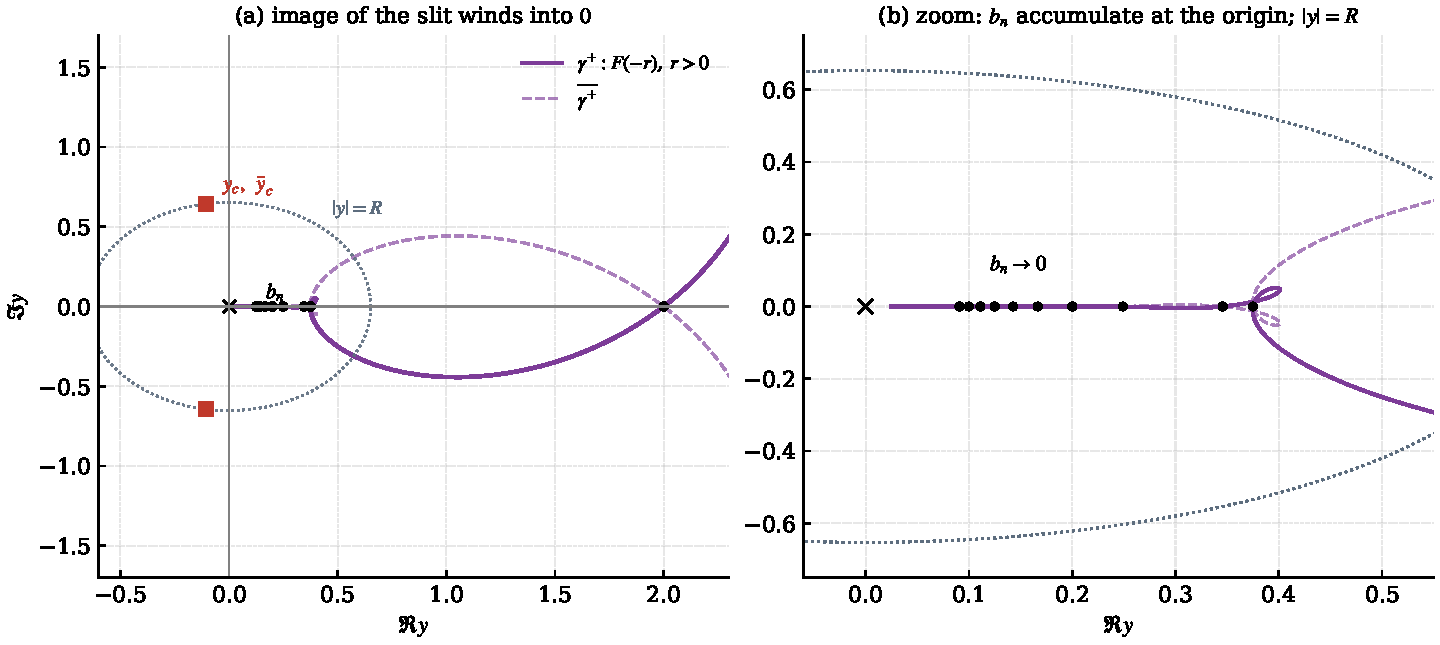
\includegraphics[width=0.98\textwidth]{figures/fig4_slit.pdf}
    \caption{(a) The slit $\gamma^{+} = f((-\infty,0))$ (solid) and its
    conjugate (dashed): the image of the negative real axis under $f$
    spirals from $-\infty + i\pi$ into the origin, crossing the real
    axis exactly at the rational points $b_{n} = (1-(-1)^{n}n^{-n})/n$
    (dots). The critical values $y_{c}$, $\overline{y_{c}}$ (squares)
    lie at distance $R = 0.6526\ldots$ from the origin (dotted circle)
    and bound the disk of convergence of the Maclaurin series
    \eqref{eq:maclaurin}. (b) Zoom near the origin: the crossings
    $b_{n}$ accumulate at $0$ alternately from both sides of $1/n$.}
    \label{fig:slit}
\end{figure}
